\section{Achieving equalized odds and equality of opportunity}
\label{sec:achieving}

We now explain how to find an equalized odds or equal opportunity
predictor $\Ytilde$ derived from a, possibly discriminatory, learned
binary predictor~$\Yhat$ or score~$R.$ We envision that~$\Yhat$ or~$R$
are whatever comes out of the existing training pipeline for the
problem at hand.  Importantly, we do not require changing the training
process, as this might introduce additional complexity, but rather
only a post-learning step.  In particular, we will construct a non-discriminating predictor which is derived from $\Yhat$ or $R$:

\begin{definition}[Derived predictor]
A predictor $\Ytilde$ is \emph{derived from a random variable $R$ and the
protected attribute~$A$} if it is a possibly randomized function of the random
variables $(R, A)$ alone.  In particular, $\Ytilde$ is independent of $X$
conditional on $(R, A).$
\end{definition}
%
The definition asks that the value of a derived predictor~$\Ytilde$
should only depend on $R$ and the protected attribute, though it may
introduce additional randomness. But the formulation of $\Ytilde$
(that is, the function applied to the values of $R$ and $A$), depends
on information about the joint distribution of $(R, A, Y).$ In other
words, this joint distribution (or an empirical estimate of it) is
required at training time in order to construct the
predictor~$\Ytilde$, but at prediction time we only have access to
values of $(R, A)$.  No further data about the underlying features
$X$, nor their distribution, is required.
%
\paragraph{Loss minimization.}
It is always easy to construct a trivial predictor satisfying
equalized odds, by making decisions independent of $X,A$ and $R$.  For
example, using the constant predictor $\Yhat=0$ or $\Yhat=1$.  The
goal, of course, is to obtain a {\em good} predictor satisfying the
condition.  To quantify the notion of ``good'', we consider a loss
function $\ell\colon\{0,1\}^2\rightarrow\mathbb{R}$ that takes a pair
of labels and returns a real number $\ell(\yhat,y)\in\mathbb{R}$ which
indicates the loss (or cost, or undesirability) of predicting $\yhat$
when the correct label is~$y.$ Our goal is then to design derived
predictors $\Ytilde$ that minimize the expected loss~$\E\ell(\Ytilde,
Y)$ subject to one of our definitions.

\subsection{Deriving from a binary predictor}
\label{sec:opt-binary}

We will first develop an intuitive geometric solution in the case where we
adjust a binary predictor~$\Yhat$ and $A$ is a binary protected attribute The
proof generalizes directly to the case of a discrete protected attribute with
more than two values. For convenience, we introduce the notation
\begin{equation}\label{eq:gamma}
\gamma_a(\Yhat) \defeq \left(
\Pr\set{ \Yhat = 1 \mid A=a, Y=0},\,
\Pr\set{ \Yhat = 1 \mid A=a, Y=1}
\right)\,.
\end{equation}
The first component of $\gamma_a(\Yhat)$ is the \emph{false positive rate} of
$\Yhat$ within the demographic satisfying $A=a.$ Similarly, the second
component is the \emph{true positive rate} of $\Yhat$ within $A=a.$
Observe that we can calculate $\gamma_a(\Yhat)$ given the
joint distribution of $(\Yhat, A, Y).$
The definitions of equalized odds and equal opportunity can be
expressed in terms of $\gamma(\Yhat)$,  as formalized in the following
straight-forward Lemma:
\begin{lemma}
\label{lem:gamma}
A predictor~$\Yhat$ satisfies:
\begin{enumerate}
\item  equalized odds if and only if
$\gamma_0(\Yhat)=\gamma_1(\Yhat),$ and
\item equal opportunity 
if and only if $\gamma_0(\Yhat)$ and
$\gamma_1(\Yhat)$ agree in the second component, i.e.,
$\gamma_0(\Yhat)_2 = \gamma_1(\Yhat)_2.$
\end{enumerate}
\end{lemma}
For $a\in\{0,1\},$ consider the two-dimensional convex polytope defined as the
convex hull of four vertices:
\begin{align}
P_a(\Yhat)  \defeq
\mathrm{convhull}\Set{ (0,0), \gamma_a(\Yhat), \gamma_a(1-\Yhat),(1,1)}
\end{align}
Our next lemma shows that $P_0(\Yhat)$ and $P_1(\Yhat)$ characterize exactly
the trade-offs between false positives and true positives that we can achieve
with any derived classifier. The polytopes are visualized
in~Figure~\ref{fig:opt-binary}.
%
\begin{lemma}
\label{lem:derived}
A predictor $\Ytilde$ is derived if and only if for all $a\in\{0,1\},$
we have $\gamma_a(\Ytilde)\in P_a(\Yhat).$
\end{lemma}
\begin{proof}
Since a derived predictor $\Ytilde$ can only depend on $(\Yhat,A)$ and these
variables are binary, the predictor $\Ytilde$ is completely described by four
parameters in~$[0,1]$ corresponding to the probabilities 
$\Pr\Set{\Ytilde =1 \mid \Yhat=\yhat,
A=a}$ for $\yhat,a\in\bits.$
Each of these parameter choices leads to one of the points in $P_a(\Yhat)$ and
every point in the convex hull can be achieved by some parameter setting.
\end{proof}
%
\begin{figure}
\begin{center}
  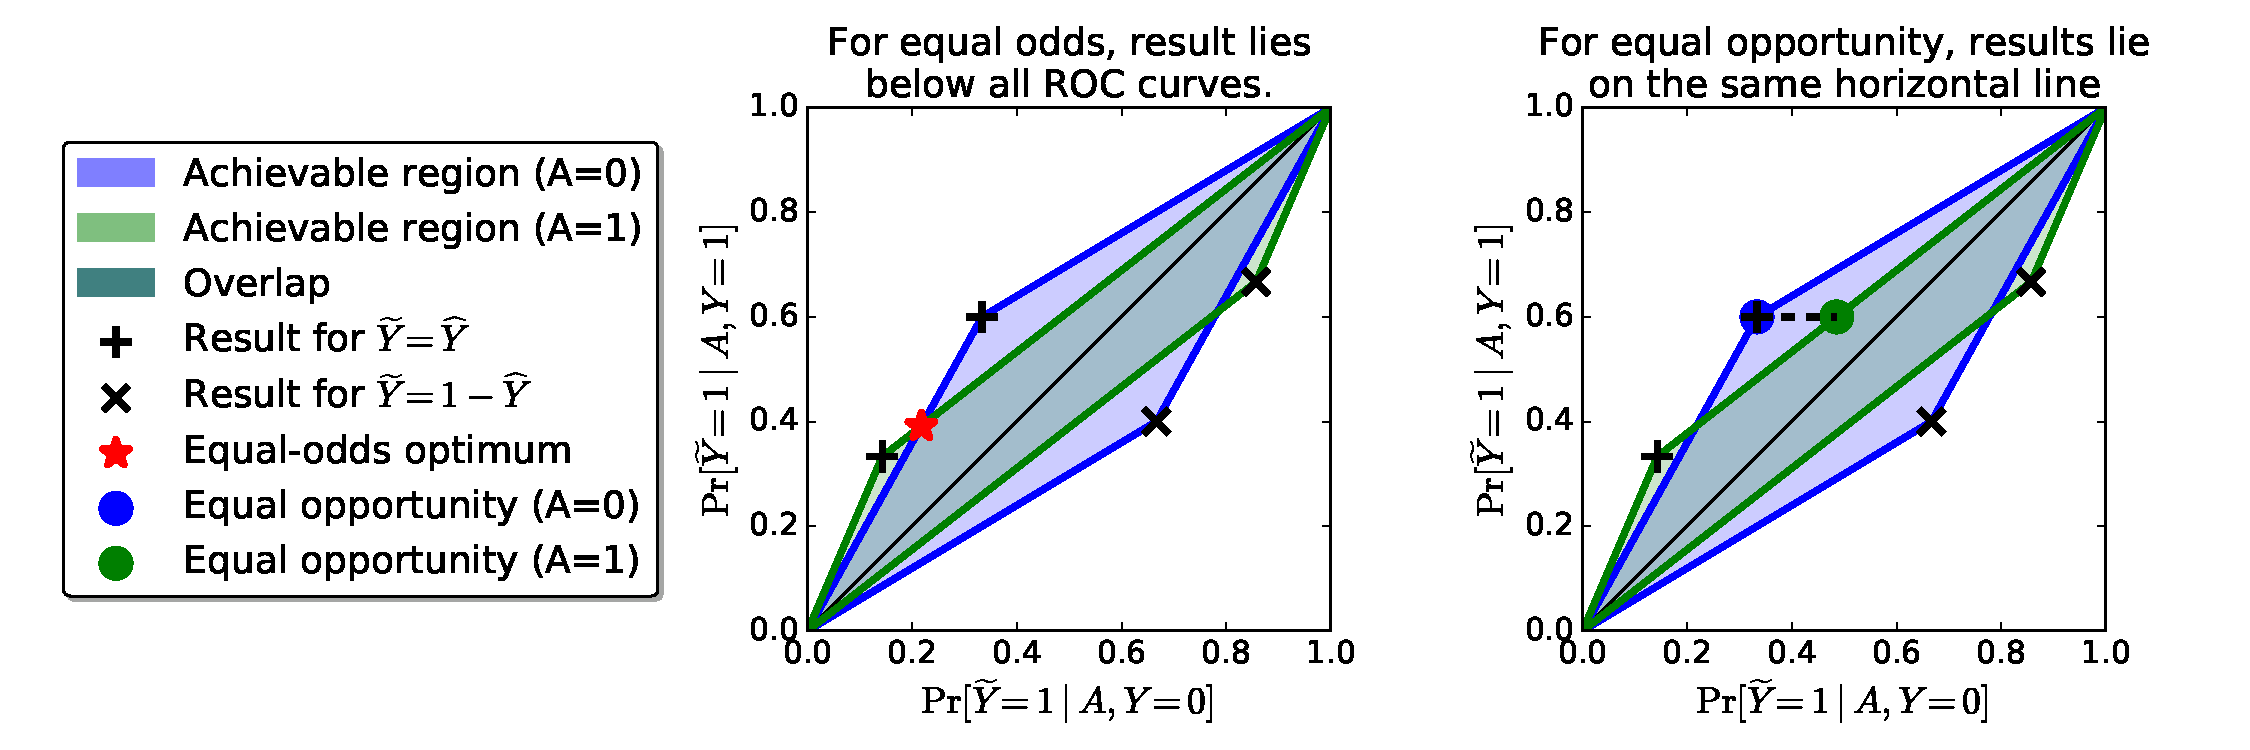
\includegraphics[width=\textwidth]{figs/binary-feasible-2}\vspace{-.3cm}
\end{center}
\caption{Finding the optimal equalized odds predictor (left), and equal
opportunity predictor (right).}
\label{fig:opt-binary}\vspace{-.5cm}
\end{figure}
%
Combining Lemma~\ref{lem:gamma} with Lemma~\ref{lem:derived}, we see that the
following optimization problem gives the optimal derived predictor with
equalized odds:
%
\begin{align}
\label{eq:opt-binary}
\min_{\Ytilde}\quad
 &\E\ell(\Ytilde, Y)\\
\mathrm{s.t.}\quad&\forall a\in\bits: \gamma_a(\Ytilde)\in P_a(\Yhat)\quad
\tag{\text{derived}}\\
& \gamma_0(\Ytilde) = \gamma_1(\Ytilde)\tag{\text{equalized odds}}%\\
\end{align}
%
Figure~\ref{fig:opt-binary} gives a simple geometric picture for the solution of
the linear program whose guarantees are summarized next.
\begin{proposition}
\label{prop:opt-binary}
The optimization problem~\eqref{eq:opt-binary} is a linear program in four
variables whose coefficients can be computed from the joint distribution of
$(\Yhat, A, Y).$ Moreover, its solution is an optimal equalized odds predictor
derived from $\Yhat$ and $A.$
\end{proposition}

\begin{proof}[Proof of Proposition~\ref{prop:opt-binary}]
The second claim follows by combining Lemma~\ref{lem:gamma} with
Lemma~\ref{lem:derived}. To argue the first claim, we saw
in the proof of Lemma~\ref{lem:derived} that a derived
predictor is specified by four parameters and the constraint region is an
intersection of two-dimensional linear constraints.
%
It remains to show that the objective function is a linear function in these
parameters. Writing out the objective, we have
\[
\E\left[\ell(\Ytilde, Y)\right]
= \sum_{y,y'\in\bits} \ell(y,y')\Pr\Set{\Ytilde=y',Y=y}\,.
\]
Further,
\begin{align*}
\Pr\Set{\Ytilde=y',Y=y}
& = \Pr\Set{\Ytilde=y',Y=y\mid \Ytilde=\Yhat}\Pr\Set{\Ytilde=\Yhat}\\
& \quad + \Pr\Set{\Ytilde=y',Y=y\mid \Ytilde\neq\Yhat}\Pr\Set{\Ytilde\neq\Yhat}\\
& = \Pr\Set{\Yhat=y',Y=y}\Pr\Set{\Ytilde=\Yhat}
+ \Pr\Set{\Yhat=1-y',Y=y}\Pr\Set{\Ytilde\neq\Yhat}\,.
\end{align*}
All probabilities in the last line that do not involve~$\Ytilde$ can be computed
from the joint distribution. The probabilities that do involve~$\Ytilde$ are each
a linear function of the parameters that specify~$\Ytilde.$
\end{proof}
%
The corresponding optimization problem for equation opportunity is the same
except that it has a weaker constraint $\gamma_0(\Ytilde)_2 =
\gamma_1(\Ytilde)_2$.
The proof is analogous to that of Proposition~\ref{prop:opt-binary}.
Figure~\ref{fig:opt-binary} explains the solution geometrically.

\subsection{Deriving from a score function}
\label{sec:opt-thresholds}

We now consider deriving non-discriminating predictors from a real
valued score~$R\in[0,1]$.  The motivation is that in many realistic
scenarios (such as FICO scores), the data are summarized by a
one-dimensional score function and a decision is made based on the
score, typically by thresholding it. Since a continuous statistic can
carry more information than a binary outcome~$Y$, we can hope to
achieve higher utility when working with~$R$ directly, rather then
with a binary predictor $\Yhat$.

A ``protected attribute blind'' way of deriving a binary predictor
from $R$ would be to threshold it, i.e.~using $\Yhat=\ind\set{R>t}$.
If $R$ satisfied equalized odds, then so will such a predictor, and
the optimal threshold should be chosen to balance false positive and
false negatives so as to minimize the expected loss.  When $R$ does
not already satisfy equalized odds, we might need to use different
thresholds for different values of $A$ (different protected groups),
i.e.~$\tilde{Y}=\ind\set{R>t_A}$.  As we will see, even this might not
be sufficient, and we might need to introduce additional randomness as
in the preceding section.

Central to our study is the ROC (Receiver Operator Characteristic)
curve of the score, which captures the false positive and true
positive (equivalently, false negative) rates at different thresholds.
These are curves in a two dimensional plane, where the horizontal axes
is the false positive rate of a predictor and the vertical axes is the
true positive rate.  As discussed in the previous section, equalized
odds can be stated as requiring the true positive and false positive
rates, ($\Pr\set{\Yhat=1 \mid Y=0,A=a},\Pr\set{\Yhat=1
  \mid Y=1,A=a}$), agree between different values of $a$ of the
protected attribute.  That is, that for all values of the protected
attribute, the conditional behavior of the predictor is at exactly the
same point in this space.  We will therefor consider the
$A$-conditional ROC curves
\[
C_a(t)\defeq\left(
\Pr\set{\Rhat > t \mid A=a, Y=0},
\Pr\set{\Rhat > t \mid A=a, Y=1}\right).
\]
Since the ROC curves exactly specify the conditional distributions $R|A,Y$,
a score function obeys equalized odds if and only if the ROC curves for all
values of the protected attribute agree, that is $C_a(t)=C_{a'}(t)$
for all values of $a$ and $t$.  In this case, any thresholding of $R$
yields an equalized odds predictor (all protected groups are at the
same point on the curve, and the same point in false/true-positive
plane).

When the ROC curves do not agree, we might choose different thresholds $t_a$
for the different protected groups.  This yields different points on
each $A$-conditional ROC curve.  For the resulting predictor to satisfy
equalized odds, these must be at the same point in the
false/true-positive plane.  This is possible only at points where all
$A$-conditional ROC curves intersect.  But the ROC curves might not all intersect
except at the trivial endpoints, and even if they do, their point of
intersection might represent a poor tradeoff between false positive
and false negatives.

As with the case of correcting a binary predictor, we can use
randomization to fill the span of possible derived predictors and
allow for significant intersection in the false/true-positive plane.
In particular, for every protected group $a$, consider the convex hull
of the image of the conditional ROC curve:
\begin{equation}\label{eq:conv-hull-threshold}
D_a  \defeq
\mathrm{convhull}\Set{ C_a(t)\colon t\in[0,1]}
\end{equation}
The definition of $D_a$ is analogous to the polytope $P_a$ in the
previous section, except that here we do not consider points below the
main diagonal (line from $(0,0)$ to $(1,1)$), which are worse than
``random guessing'' and hence never desirable for any reasonable loss
function.  

\paragraph{Deriving an optimal equalized odds threshold predictor.}
Any point in the convex hull~$D_a$ represents the false/true positive
rates, conditioned on $A=a$, of a randomized derived predictor based
on $R$.  In particular, since the space is only two-dimensional, such
a predictor~$\tilde Y$ can always be taken to be a mixture of two threshold
predictors (corresponding to the convex hull of two points on the
ROC curve). Conditional on $A=a,$ the predictor $\tilde Y$ behaves as
\[
\tilde{Y} = \ind\set{R>T_a}\,,
\]
where $T_a$ is a randomized threshold assuming the
value~$\underline{t}_a$ with probability~$\underline{p}_a$ and the
value~$\overline{t}_a$ with probability~$\overline{p}_a$.  In other
words, to construct an equalized odds predictor, we should choose a
point in the intersection of these convex hulls,
$\gamma=(\gamma_0,\gamma_1) \in \cap_a D_a$, and then for each
protected group realize the true/false-positive rates $\gamma$ with a
(possible randomized) predictor $\tilde{Y}|(A=a) = \ind\set{R>T_a}$
resulting in the predictor $\tilde{Y} = \Pr\ind\set{R>T_A}$.  For each
group~$a$, we either use a fixed threshold $T_a=t_a$ or a mixture of
two thresholds $\underline{t}_a<\overline{t}_a$.  In the latter case,
if $A=a$ and $R<\underline{t}_a$ we always set $\tilde{Y}=0$, if
$R>\overline{t}_a$ we always set $\tilde{Y}=1$, but if
$\underline{t}_a<R<\overline{t}_a$, we flip a coin and set
$\tilde{Y}=1$ with probability $\underline{p}_a$.
%
\begin{figure}
\begin{center}
  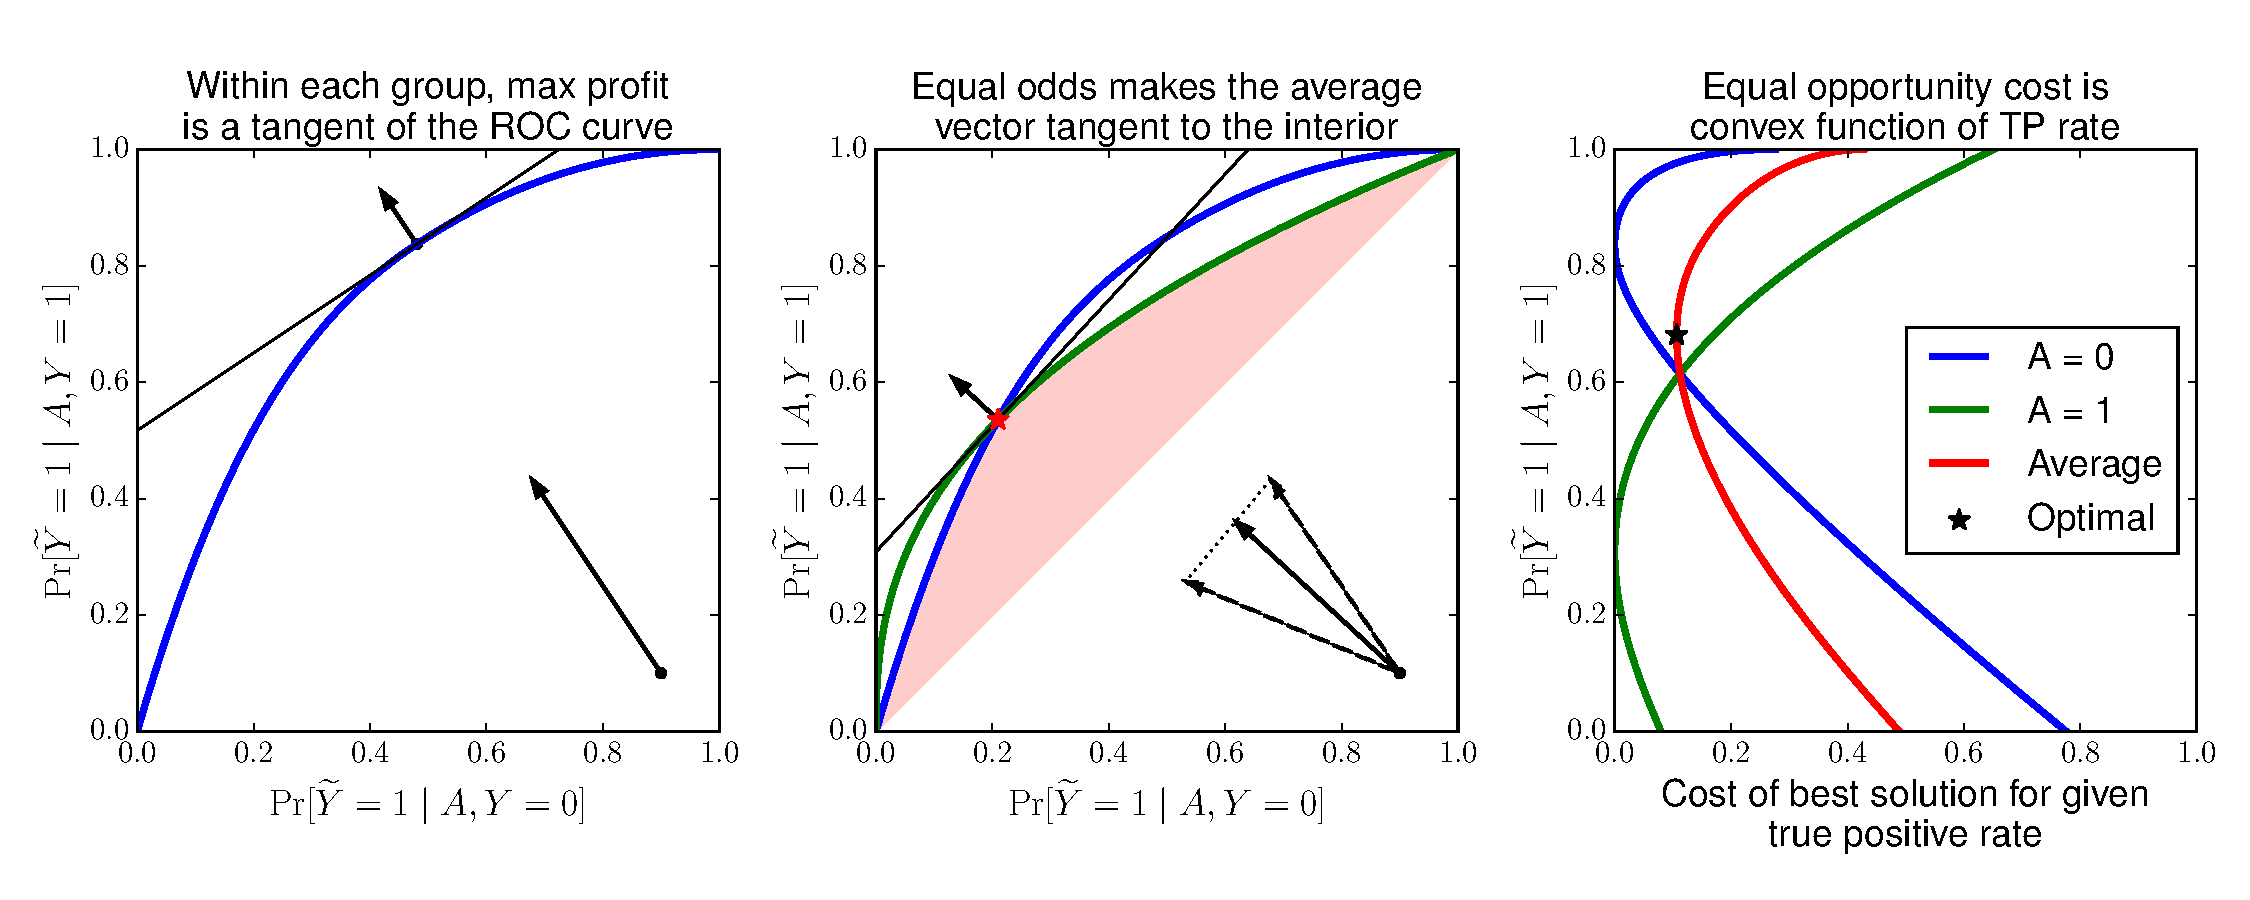
\includegraphics[width=\textwidth]{figs/threshold-example}\vspace{-.5cm}
\end{center}
\caption{Finding the optimal equalized odds threshold predictor
  (middle), and equal opportunity threshold predictor (right).  For
  the equal opportunity predictor, within each group the cost for a
  given true positive rate is proportional to the horizontal gap between the ROC
  curve and the profit-maximizing tangent line (i.e., the two curves
  on the left plot), so it is a convex function of the true positive
  rate (right).  This lets us optimize it efficiently with ternary search.}
\label{fig:opt-binary-thresholds}\vspace{-.5cm}
\end{figure}

The feasible set of false/true positive rates of possible equalized
odds predictors is thus the intersection of the areas under the
$A$-conditional ROC curves, and above the main diagonal (see Figure
\ref{fig:opt-binary-thresholds}).  Since for any loss function the optimal
false/true-positive rate will always be on the upper-left boundary of
this feasible set, this is effectively the ROC curve of the equalized odds
predictors.  This ROC curve is the pointwise minimum of all $A$-conditional
ROC curves.  The performance of an equalized odds predictor is thus
determined by the minimum performance among all protected groups.
Said differently, requiring equalized odds incentivizes the learner to
build good predictors for {\em all} classes.
%
For a given loss function, finding the optimal tradeoff amounts to
optimizing (assuming w.l.o.g.~$\ell(0,0)=\ell(1,1)=0$):
\begin{equation}
  \label{eq:opt-obj-R}
  \min_{\forall a\colon \gamma\in D_a} \gamma_0\ell(1,0)+(1-\gamma_1)\ell(0,1)
\end{equation}
This is no longer a linear program, since $D_a$ are not polytopes, or
at least are not specified as such.  Nevertheless,
\eqref{eq:opt-obj-R} can be efficiently optimized numerically using
ternary search.

\paragraph{Deriving an optimal equal opportunity threshold predictor.}
The construction follows the same approach except that there is one fewer constraint.
We only need to find points on the conditional ROC curves that have the same
true positive rates in both groups. Assuming continuity of the conditional ROC
curves, this means we can always find points on the boundary of the
conditional ROC curves. In this case, no randomization is necessary. The
optimal solution corresponds to two deterministic thresholds, one for each
group. As before, the optimization problem can be solved efficiently using
ternary search over the target true positive value. Here we use, as
Figure~\ref{fig:opt-binary-thresholds} illustrates, that the cost of the best
solution is convex as a function of its true positive rate.

\section{Bayes optimal predictors}
\label{sec:bayes}
%
In this section, we develop the theory a theory for non-discriminating
Bayes optimal classification.  We will first show that a Bayes optimal
equalized odds predictor can be obtained as an derived threshold
predictor of the Bayes optimal regressor. Second, we quantify the loss
of deriving an equalized odds predictor based on a regressor that
deviates from the Bayes optimal regressor. This can be used to justify
the approach of first training classifiers without any fairness
constraint, and then deriving an equalized odds predictor in a second
step.
%
\begin{definition}[Bayes optimal regressor]
  Given random variables $(X,A)$ and a target variable~$Y,$ the
  \emph{Bayes optimal regressor} is
  $R=\arg\min_{r(x,a)}\E\left[(Y-r(X,A))^2\right]=r^*(X,A)$ with
  $r^*(x,a) = \E[Y \mid X=x, A=a].$
\end{definition}

The Bayes optimal classifier, for any proper loss, is then a threshold
predictor of~$R,$ where the threshold depends on the loss function
(see, e.g., \cite{Wasserman10}).  We will extend this result to the
case where we additionally ask the classifier to satisfy an oblivious
property, such as our non-discrimination properties.
%
\begin{proposition}
\label{lem:oblivious-optimal}
\label{prop:oblivious-optimal} For any source distribution over
$(Y,X,A)$ with Bayes optimal regressor $R(X,A)$, any loss function,
and any oblivious property $C$, there exists a predictor $Y^*(R,A)$
such that:
\begin{enumerate}
\item $Y^*$ is an optimal predictor satisfying~$C$.  That is,
  $\E\ell(Y^*,Y)\leq\E\ell(\Yhat,Y)$ for any predictor $\Yhat(X,A)$
  which satisfies~$C$.
\item $Y^*$ is derived from $(R,A).$
\end{enumerate}
\end{proposition}
%
\begin{figure}[ht]
\begin{center}
  \begin{tikzpicture}[->,auto, semithick, scale=1,every node/.style={scale=1}]
    \tikzset{var/.style={draw=black,circle,minimum size=0.7cm, inner sep=0pt}};
    \node[var] (A) {$A$};
    \node[var, left of=A] (X) {$X$};
    \node[var, right of=A] (X2) {$X'$};
    \node[var] at ($ (A)!.5!(X) +  (0, 1) $) (R) {$R$};
    \node[var] at ($ (A)!.5!(X) -  (0, 1) $) (Yh) {$\Yhat$};
    \node[var, right of=R] (Y) {$Y$};
    \node[var, right of=Yh] (Ys) {$Y^*$};
    {
      \path (X) edge (R)
            edge (Yh)
        (A) edge (R)
            edge (X)
            edge (Yh)
            edge (Ys)
            edge (X2)
        (R) edge (X2)
            edge (Y)
        (X2) edge (Ys)
        (X) edge (Yh)
        ;
      }
    \end{tikzpicture}
\end{center}
    \caption{Graphical model for the proof of Proposition~\ref{prop:oblivious-optimal}.}
\label{fig:graphmodel}
\end{figure}
%
\begin{proof}
  Consider an arbitrary classifier $\Yhat$ on the attributes $(X,A)$,
  defined by a (possibly randomized) function $\Yhat=f(X,A).$ Given
  $(R=r, A=a)$, we can draw a fresh $X'$ from the distribution $(X
  \mid R=r, A=a)$, and set $Y^* = f(X', a)$.  This satisfies (2).
  Moreover, since $Y$ is binary with expectation $R$, $Y$ is
  independent of $X$ conditioned on $(R, A)$.  Hence $(Y, X, R, A)$
  and $(Y, X', R, A)$ have identical distributions, so $(Y^*, A, Y)$ and
  $(\Yhat, A, Y)$ also have identical distributions.  This implies $Y^*$
  satisfies (1) as desired.
\end{proof}


\begin{corollary}[Optimality characterization]
\label{cor:bayes-opt-fair}
An optimal equalized odds predictor can be derived from the Bayes
optimal regressor~$R$ and the protected attribute~$A.$ The same is true for
an optimal equal opportunity predictor.
\end{corollary}

\subsection{Near optimality}
%
We can furthermore show that if we can approximate the (unconstrained)
Bayes optimal regressor well enough, then we can also construct a
nearly optimal non-discriminating classifier.

To state the result, we introduce the following distance measure on random
variables.
\begin{definition}
We define the \emph{conditional Kolmogorov distance}
between two random variables $R,R'\in[0,1]$ in the same probability space
as~$A$ and~$Y$ as:
\begin{equation}
d_{\mathrm{K}}(R, R')\defeq
\max_{a,y\in\{0,1\}} \sup_{t\in[0,1]}
\left|\Pr\Set{R > t\mid A=a, Y=y}
- \Pr\Set{R' > t\mid A=a, Y=y}
\right|\,.
\end{equation}
\end{definition}
Without the conditioning on $A$ and $Y,$ this definition coincides with the
standard Kolmogorov distance. Closeness in Kolmogorov distance is a rather weak
requirement. We need the slightly stronger condition that the Kolmogorov
distance is small for each of the four conditionings on $A$ and $Y.$ This
captures the distance between the restricted ROC curves, as formalized next.
%
\begin{lemma}\label{lem:pythagoras}
Let $R, R'\in[0,1]$ be random variables in the same probability space as $A$ and
$Y.$ Then, for any point $p$ on a restricted ROC curve of $R,$ there is a point
$q$ on the corresponding restricted ROC curve of $R'$ such that
$\|p-q\|_2\le\sqrt{2}\cdot d_K(R, R').$
\end{lemma}
\begin{proof}
Assume the point $p$ is achieved by thresholding $R$ at $t\in[0,1].$ Let $q$ be
the point on the ROC curve achieved by thresholding $R'$ at the same threshold
$t'.$ After applying the definition to bound the distance in each coordinate,
the claim follows from Pythagoras' theorem.
\end{proof}
%
We can now show that an equalized odds predictor derived from a nearly optimal
regressor is still nearly optimal among all equal odds predictors, while
quantifying the loss in terms of the conditional Kolmogorov distance.
%
\begin{theorem}[Near optimality]
\label{cor:near-optimality}
\label{thm:near-optimality}
Assume that~$\ell$ is a bounded loss function, and let $\Rhat\in[0,1]$ be an
arbitrary random variable. Then, there is an optimal equalized odds
predictor~$Y^*$ and an equalized odds predictor $\Yhat$ derived from~$(\Rhat, A)$
such that
\[
\E\ell(\Yhat, Y)\le \E\ell(Y^*,Y) + 2\sqrt{2}\cdot d_{\mathrm{K}}(\Rhat,R^*)\,,
\]
where $R^*$ is the Bayes optimal regressor.  The same claim is true for equal
opportunity.
\end{theorem}

\begin{proof}[Proof of Theorem~\ref{thm:near-optimality}]
We prove the claim for equalized odds. The case of equal opportunity is
analogous.

Fix the loss function~$\ell$ and the regressor~$\Rhat.$ Take $Y^*$ to be the
predictor derived from the Bayes optimal regressor~$R^*$ and~$A.$ By
Corollary~\ref{cor:bayes-opt-fair}, we know that this is an optimal equalized
odds predictor as required by the lemma.
It remains to construct a derived equalized odds predictor~$\Yhat$ and relate
its loss to that of $Y^*.$

Recall the optimization problem for defining the optimal derived equalized odds predictor.
Let $\widehat D_a$ be the constraint region defined by $\Rhat.$ Likewise,
let $D_a^*$ be
the constraint region under $R^*.$ The optimal classifier~$Y^*$ corresponds to a
point $p^*\in D_0^*\cap D_1^*.$ As a consequence of Lemma~\ref{lem:pythagoras},
we can find (not necessarily identical) points
$q_0\in \widehat D_0$ and $q_1\in \widehat D_1$ such that for all $a\in\{0,1\},$
\[
\|p^*-q_a\|_2\le \sqrt{2}\cdot d_{\mathrm{K}}(\Rhat, R^*)\,.
\]
We claim that this means we can also find a feasible
point $q\in \widehat D_0\cap \widehat D_1$ such that
\[
\|p^*-q\|_2\le 2\cdot d_{\mathrm{K}}(\Rhat, R^*)\,.
\]
To see this, assume without loss of generality that the first coordinate of
$q_1$ is greater than the first coordinate of $q_0,$ and that all points
$p^*,q_0,q_1$ lie
above the main diagonal. By definition of $\widehat D_1,$ we know that the
entire line segment~$L_1$ from $(0, 0)$ to $q_1$ is contained in $\widehat
D_1.$ Similarly, the entire line segment~$L_0$ between $q_0$ and $(1,1)$ is
contained in $\widehat D_0.$ Now, take $q\in L_0\cap L_1.$ By construction,
$q\in \widehat D_0\cap\widehat D_1$ defines a classifier $\Yhat$ derived from
$\Rhat$ and~$A.$ Moreover,
\[
\|p^*-q\|_2^2 \le \|p^*-q_0\|_2^2 + \|p^*-q_0\|_2^2
\le 4\cdot d_{\mathrm{K}}(\Rhat, R^*)^2\,.
\]
Finally, by assumption on the loss function,
there is a vector $v$ with $\|v\|_2\le\sqrt{2}$ such that $\E\ell(\Yhat,
Y)=\langle v, q\rangle$ and $\E\ell(Y^*,Y)=\langle v, p^*\rangle.$ Applying
Cauchy-Schwarz,
\[
\E\ell(\Yhat,Y)-\E\ell(Y^*,Y)
= \langle v, q-p^*\rangle\le \|v\|_2\cdot\|q-p^*\|_2
\le 2\sqrt{2}\cdot d_{\mathrm{K}}(\Rhat, R^*)\,.
\]
This completes the proof.
\end{proof}
